% Copyright (C) 2011 Thomas L. Kula
% All Rights Reserved
%
% See the file LICENSE for license terms.
\documentclass[12pt]{article}
\usepackage{graphicx}
\usepackage{rotating}
\usepackage{fix-cm}
\usepackage{multirow}
\setlength{\paperwidth}{5.5in}
\setlength{\paperheight}{8.5in}
\setlength{\textheight}{7.45in}
\setlength{\topmargin}{-1.0in}
\setlength{\oddsidemargin}{-0.5in}
\setlength{\evensidemargin}{-0.5in}
\setlength{\textwidth}{4.0in}
\setlength{\parindent}{0in}
\setlength{\parskip}{3mm}
\usepackage[print]{booklet} \nofiles
\source{\magstep0}{5.5in}{8.5in}
\target{\magstep0}{11in}{8.5in}
\setpdftargetpages
\pagestyle{empty}
\begin{document}


\begin{center}
{\fontsize{36}{48}\selectfont \textsc{Haiku a Day }}
\end{center}

\vspace*{3.5cm}

{\fontsize{20}{40}\selectfont 

The end of the year

Relaxing, yet full of things

Appointment book full

}

\vspace*{5.0cm}
\begin{center}
{\large{Issue 77: November 2011}} \\[5mm]
{\fontsize{8}{8}\selectfont  \textsc{ St. Joshua Norton Press }} \\[1mm]
{\fontsize{6}{6}\selectfont Mathom House by the Cloisters \textbar The People's Republic of Ames }
\end{center}


\newpage

Sorry for the delay on this issue, getting settled in, unpacking,
and finishing up {\em Late Night Thinking 8: Gumption} has occupied
most of my time. But it's all good, LNT comes out next week, I'm
mostly unpacked, and I finally uploaded moving photos:

{\tt kula.tproa.net/photos/2011/moving-to-nyc/ }

Until next month, and next year, enjoy.


--- Thomas

http://kula.tproa.net/had/ \\
kula@tproa.net

Download this and previous HADs at the website, so you can
print out your own (DIY, yeah!) or if you want me to send
you one, send me your address, and maybe a stamp if you
are feeling nice. Or send me something you've made ---
trades always appreciated, postcards are nice too.

\vfill

1 November 2011

The list grows longer \\
Of things I must go pick up \\
This weekend, the store

2 November 2011

Hear the traffic go \\
Even at night, the city \\
Moves with urgency

\newpage

3 November 2011

Sink faucet, dripping \\
Handle's delicate dancing  \\
Try to make it stop

4 November 2011

Like a child, lost \\
Had that pen for many months \\
Used it, forgot it

5 November 2011

The gnome grows absurd \\
Without a lawn, it suffers \\
By a flower pot

6 November 2011

That lamp works, makes light \\
The switch, broken, always on \\
Useless, not enough

7 November 2011

Under dark corners \\
The dust of a thousand years \\
Silently waiting

8 November 2011

New box of paper \\
What joy will you bring to us \\
Five thousand canvas

9 November 2011

Apartment basement \\
Holding many secret things \\
I seek the laundry

\newpage

10 November 2011

Gas hisses. Release. \\
Chilled water and a few shakes. \\
Press lever for fun.

11 Novemeber 2011

One hundred year grime \\
Tunnels the color of mud \\
Grease and gunk built up

12 November 2011

With a wary eye \\
At the apartment fuse box \\
Plugging more stuff in

13 November 2011

How long did that take \\
Weird scaly thing up above \\
Found in my bathroom

14 November 2011

There, dully thudding \\
A monster behind my eyes \\
Begone, foul demon

15 November 2011

The simple joy found \\
When I can walk to errands \\
During my lunch break

16 November 2011

Spy a lonely bench \\
Huddled alone by a light \\
Nobody sitting

\newpage

17 November 2011

Subterranean \\
Highways, stretching the city \\
Going here and there

18 November 2011
 
Yearning of a tree \\
To feel sunlight and water \\
It bends, so slowly

19 November 2011

Not broken, just off \\
A few fine adjustments fix \\
What was once rubbish

20 November 2011

A slip, and it breaks \\
Shards of glass, the kitchen sink \\
Shoulda bought plastic

21 November 2011

Like a hug, reverse \\
A towel fresh from the dryer \\
Wrapped bundle of warmthh

22 November 2011

Done now with shopping \\
And I should put things away \\
Recliner beckons

23 November 2011

Anticipation \\
Giddy thoughts growing, waiting \\
Release an idea

\newpage

24 November 2011

Planing for the day \\
Lots of food, taking some naps \\
And Lord of the Rings

25 November 2011

Fuck fuck fuck fuck fuck \\
What the hell is wrong with you \\
Why do you hate me, back?

26 November 2011

Out of bed today \\
For maybe twenty minutes \\
I curse all pinched nerves

27 November 2011

Stuck in bed all day \\
Isn't as fun as it sounds \\
Some day I'll get up

28 November 2011

To the door! Made it! \\
The journey to work and back \\
An epic mission

29 November 2011

A quiet globe glows \\
Casting light upon the ground \\
A tree loses leaves

30 November 2011

Always crave pizza \\
I should be eating healthy \\
But there's pizza, man


\newpage

\begin{center}
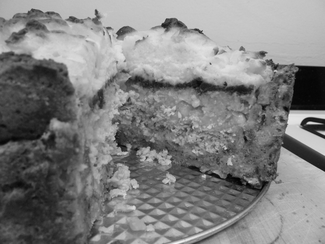
\includegraphics[width=325pt]{tday-pie.png}

Thanksgiving Pie, 24 November 2011 \\
{\tt kula.tproa.net/photos/2011/11/20111124-thanksgiving-pie/ }
\end{center}

\newpage

\thispagestyle{empty}
\vspace*{12cm}
\begin{sideways}
\Large{St. Joshua Norton Press}
\end{sideways}
\begin{sideways}
\Large{PO Box 250138}
\end{sideways}
\begin{sideways}
\Large{New York NY 10025}
\end{sideways}


\end{document}


